\documentclass{beamer}
\usepackage[latin1]{inputenc}

\usetheme{Madrid}
\usecolortheme{default}
\usepackage{amsmath}
\usepackage{amssymb,amsfonts,amsthm}
\usepackage{txfonts}
\usepackage{tkz-euclide}
\usepackage{listings}
\usepackage{adjustbox}
\usepackage{array}
\usepackage{tabularx}
\usepackage{gvv}
\usepackage{lmodern}
\usepackage{circuitikz}
\usepackage{tikz}
\usepackage{graphicx}
\usepackage{gensymb}
\usepackage{physics}

\setbeamertemplate{page number in head/foot}[totalframenumber]

\usepackage{tcolorbox}
\tcbuselibrary{minted,breakable,xparse,skins}



\definecolor{bg}{gray}{0.95}
\DeclareTCBListing{mintedbox}{O{}m!O{}}{%
  breakable=true,
  listing engine=minted,
  listing only,
  minted language=#2,
  minted style=default,
  minted options={%
    linenos,
    gobble=0,
    breaklines=true,
    breakafter=,,
    fontsize=\small,
    numbersep=8pt,
    #1},
  boxsep=0pt,
  left skip=0pt,
  right skip=0pt,
  left=25pt,
  right=0pt,
  top=3pt,
  bottom=3pt,
  arc=5pt,
  leftrule=0pt,
  rightrule=0pt,
  bottomrule=2pt,
  toprule=2pt,
  colback=bg,
  colframe=orange!70,
  enhanced,
  overlay={%
    \begin{tcbclipinterior}
    \fill[orange!20!white] (frame.south west) rectangle ([xshift=20pt]frame.north west);
    \end{tcbclipinterior}},
  #3,
}
\lstset{
    language=C,
    basicstyle=\ttfamily\small,
    keywordstyle=\color{blue},
    stringstyle=\color{orange},
    commentstyle=\color{green!60!black},
    numbers=left,
    numberstyle=\tiny\color{gray},
    breaklines=true,
    showstringspaces=false,
}
\title{4.7.11}
\date{13th september, 2025}
\author{Vishwambhar - EE25BTECH11025}

\begin{document}

\frame{\titlepage}
\begin{frame}{Question}
Show that the path of a moving point such that its distance from two lines  $3x-2y=5$ and $3x+2y=5$ are equal is a straight line.\\
\end{frame}

\begin{frame}{Given}
Given line equations can be written as:
\begin{align}
    \vec{n}_1^\top\vec{x}=c_1\\
    \vec{n}_1=\myvec{3\\-2};c_1=5\\
    \vec{n}_2^\top\vec{x}=c_2\\
    \vec{n}_2=\myvec{3\\2};c_2=5
\end{align}

let the point equidistant from the given lines be:
\begin{align}
    \vec{P}=\myvec{x\\y}
\end{align}
\end{frame}

\begin{frame}{Proof}
From distance formula:
\begin{align}
    d_1=\frac{|\vec{n}_1^\top\vec{P}-c_1|}{||\vec{n}_1||}\\
    d_2=\frac{|\vec{n}_2^\top\vec{P}-c_2|}{||\vec{n}_2||}\\
    \because d_1=d_2\\
    \frac{|\vec{n}_1^\top\vec{P}-c_1|}{||\vec{n}_1||}=\frac{|\vec{n}_2^\top\vec{P}-c_2|}{||\vec{n}_2||}\\
    \because ||\vec{n}_1||=||\vec{n}_2||=\sqrt{3^2+2^2}=\sqrt{13}\\
    \vec{n}_1^\top\vec{P}-c_1=\pm\brak{\vec{n}_2^\top\vec{P}-c_2}
\end{align}
\end{frame}

\begin{frame}{checking}
First, by taking $+$:
\begin{align}
    \vec{n}_1^\top\vec{P}-c_1=+\brak{\vec{n}_2^\top\vec{P}-c_2}\\
    \vec{n}_1^\top\vec{P}-\vec{n}_2^\top\vec{P}=c_1-c_2\\
    \brak{\vec{n}_1-\vec{n}_2}^\top\vec{P}=c_1-c_2\\
    \myvec{0&-4}\vec{P}=0
\end{align}

Now by taking $-$:
\begin{align}
    \vec{n}_1^\top\vec{P}-c_1=-\brak{\vec{n}_2^\top\vec{P}-c_2}\\
    \vec{n}_1^\top\vec{P}+\vec{n}_2^\top\vec{P}=c_1+c_2\\
    \brak{\vec{n}_1+\vec{n}_2}^\top\vec{P}=c_1+c_2\\
    \myvec{6&0}\vec{P}=10
\end{align}
\end{frame}

\begin{frame}{Conclusion}
Since equations (15) and (19) are in the form of line equation $\vec{n}^\top\vec{x}=c$, the given path of the moving point is a line.
\end{frame}


\begin{frame}[fragile]
    \frametitle{C Code}
    \begin{lstlisting}
#include <stdio.h>

int vector1[2]={3, -2};
int constant1[1]={5};
int vector2[2]={3, 2};
int constant2[1]={5};

void give_data(double *points){
    points[0] = vector1[0];points[1] = vector1[1];
    points[2] = constant1[0];
    points[3] = vector2[0]; points[4] = vector2[1];
    points[5] = constant2[0];
}
    \end{lstlisting}
\end{frame}

\begin{frame}[fragile]
    \frametitle{C Code}
    \begin{lstlisting}
void give_findata(double *points2){ 
    double finalvector1[2]; double finalvector2[2]; 
    double finalconstant1; double finalconstant2;
    for(int i = 0; i<2; i++){
        finalvector1[i] = vector1[i] - vector2[i];
        finalvector2[i] = vector1[i] + vector2[i];
    }  
    finalconstant1 = constant1[0] - constant2[0];
    finalconstant2 = constant1[0] + constant2[0];
    points2[0] = finalvector1[0];points2[1] = finalvector1[1];
    points2[2] = finalconstant1;
    points2[3] = finalvector2[0]; points2[4] = finalvector2[1];
    points2[5] = finalconstant2;
}
    \end{lstlisting}
\end{frame}

\begin{frame}[fragile]
    \frametitle{Python Code 1}
    \begin{lstlisting}
import ctypes as ct

lib = ct.CDLL("./problem.so")
lib.give_data.argtypes = [ct.POINTER(ct.c_double)]
lib.give_findata.argtypes = [ct.POINTER(ct.c_double)]

points = ct.c_double*8
data = points()
lib.give_data(data)
finpoints = ct.c_double*8
findata = finpoints()
lib.give_findata(findata)

def send_data():
    return data, findata 
    \end{lstlisting}
\end{frame}

\begin{frame}[fragile]
    \frametitle{Python Code 2}
    \begin{lstlisting}
import matplotlib.pyplot as plt
import numpy as np
from call import send_data
data, findata = send_data()
a = np.linspace(-10, 10, 100)
b = ((data[0]*a)-data[2])/(-data[1])
A = np.linspace(-10, 10, 100)
B = ((-data[3]*A)+data[5])/data[4]
y = np.linspace(-10, 10, 100)
x = ((findata[4]*y)-findata[5])/(-findata[3])
X = np.linspace(-10, 10, 100)
Y = ((findata[0]*X)-findata[2])/(-findata[1])
    \end{lstlisting}
\end{frame}

\begin{frame}[fragile]
    \frametitle{Python Code 2}
    \begin{lstlisting}
plt.plot(a, b, 'r-') 
plt.plot(A, B, 'r-')
plt.plot(x, y, 'k-')
plt.plot(X, Y, 'k-')
plt.text(10, 12.3, "3x-2y=5", fontsize=10, color='black')
plt.text(-8.3, 15, "3x+2y=5", fontsize=10, color='black')
plt.text(15.2, -0.06, "y=0", fontsize=10, color='black')
plt.text(1.6, 14.6, "x=10/6", fontsize=10, color='black')
plt.xlabel('X-axis')
plt.ylabel('Y-axis')
plt.axis('equal')
plt.grid(True)
plt.savefig("../figs/plot.png")
plt.show()    \end{lstlisting}
\end{frame}

\begin{frame}{Plot}
    \begin{figure}
        \centering
        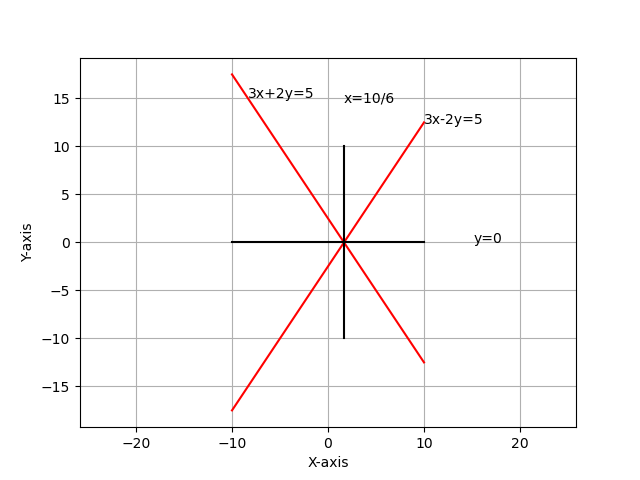
\includegraphics[width=0.5\columnwidth]{../figs/plot.png}
        \caption{Plot of given lines and path of the moving points}
        \label{fig:fig}
    \end{figure}
\end{frame}




\end{document}
